\subsection{Database Arkitektur}

I oprettelsen af systemets database skal der tages hånd om, hvordan kommunikationen skal foregå imellem systemets segmenter, samt databasens funktionalitet. Her er der blevet besluttet at der anvendes en DAL, der fungerer ved at hver gang databasen skal kontaktes, så foregår det igennem denne. Yderligere vil denne DAL også simplificere kommunikationen mellem databasen og Back-End.

\begin{figure}[H]
\centering
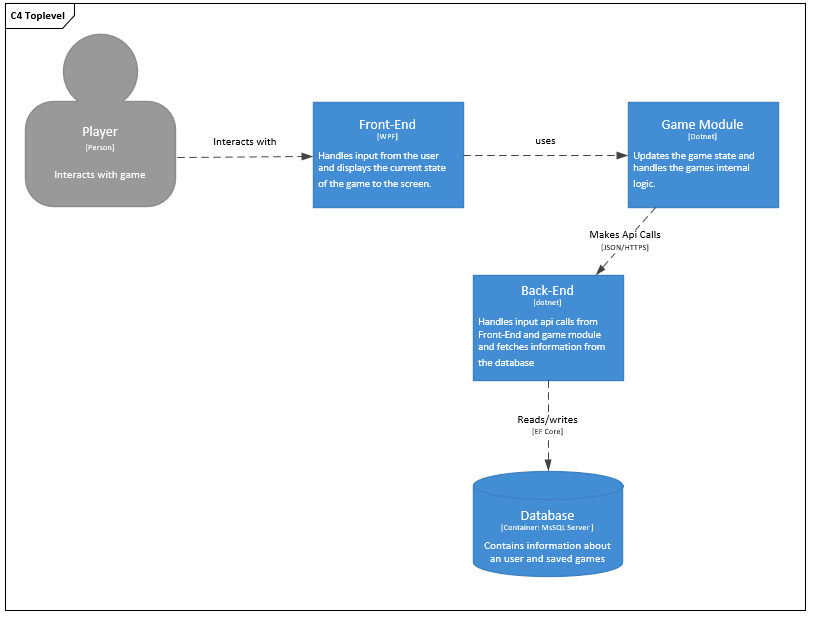
\includegraphics[width = \textwidth]{02-Body/Images/C4TopLvlDB}
\caption{C4 top level diagram, som viser kommunikation mellem systemets segmenter}
\label{fig:C4TopLvlDB}
\end{figure}

Måden kommunikationen vil foregå igennem systemet vises på \autoref{fig:C4TopLvlDB}. Her ses der at en bruger interagere med Front-End, data går videre til Game Module, som kommunikere med Back-End, hvor der til sidst enten bliver skrevet til databasen eller hentet data fra databasen
For at illustrere databasens funktionalitet er der blevet dannet sekvensdiagrammer, som viser hvordan databasen vil kunne gemme et spil og hente et gemt spil.

\begin{figure}[H]
\centering
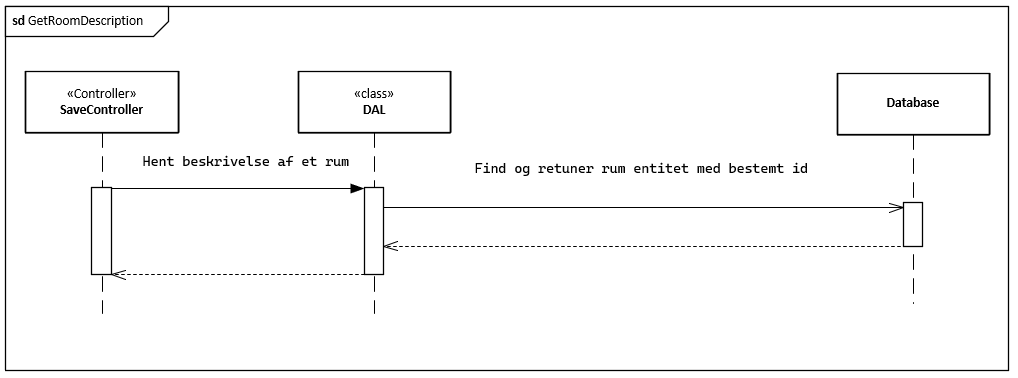
\includegraphics[width = \textwidth]{02-Body/Images/RoomDescriptionsDB.PNG}
\caption{Sekvensdiagram for hvordan rum beskrivelser vil blive hente fra databasen af SaveController}
\label{fig:RoomDescriptionsDB}
\end{figure}

I \autoref{fig:RoomDescriptionsDB} ses diagrammet GetRoomDescription ses der, hvordan kommunikationen ville foregå for at hente rum beskrivelsen. Her ses der at SaveController, fra Back-End, går til DAL, som så henter rum beskrivelsen fra databasen, og herefter returneres dataene fra databasen til DAL og så fra DAL til SaveController.

\begin{figure}[H]
\centering
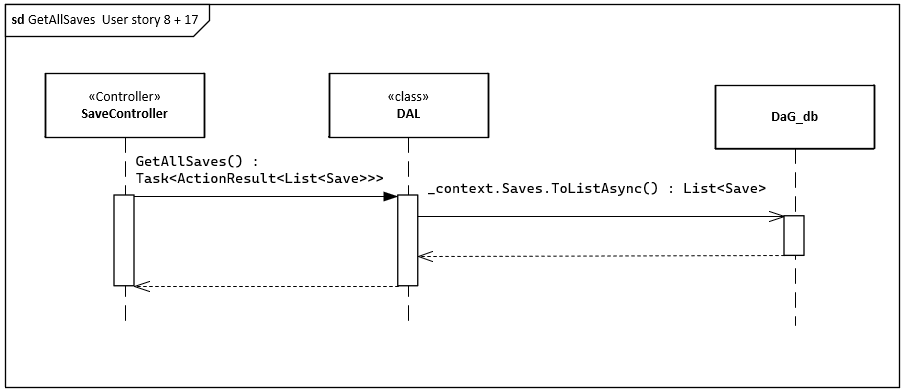
\includegraphics[width = \textwidth]{02-Body/Images/GetAllSavesDB.PNG}
\caption{Sekvensdiagram for User story 8 + 17: GetAllSaves, i relation til hentet data fra database}
\label{fig:GetAllSavesDB}
\end{figure}

I figuren \autoref{fig:GetAllSavesDB} ses diagrammet GetAllSaves foregår kommunikation på samme måde som ved at hente rum beskrivelser. Forskellen her er dog at der i stedet for hentes en list af alle gemte spil.

\begin{figure}[H]
\centering
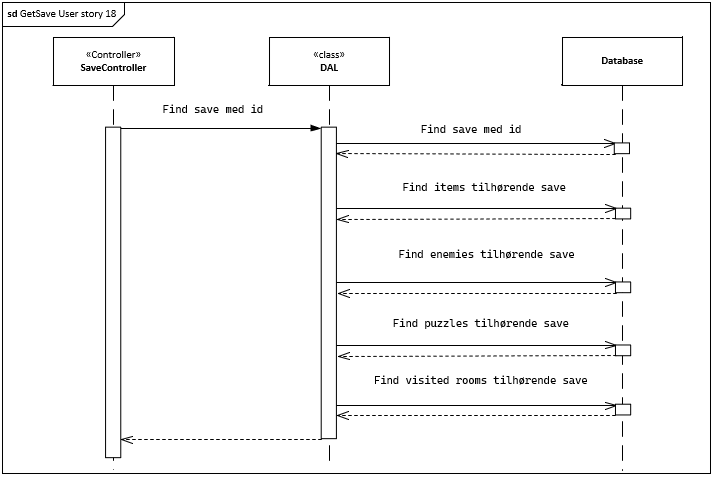
\includegraphics[width = \textwidth]{02-Body/Images/GetSaveDB.PNG}
\caption{Sekvensdiagram for User story 18: GetAllSaves, i relation til hentet data fra specifikt gemt spil fra database}
\label{fig:GetSaveDB}
\end{figure}

I \autoref{fig:GetSaveDB} ses diagrammet GetSave ses der hvordan et specifikt gemt spil hentes. Her ses der at dataene igen går først igennem DAL. Et gemt spil vil have et ID, som der kan anvendes til at finde de korresponderende værdier som dette gemte spil har. Her ses der at der vil findes items, enemies, puzzles og hvilke rum en spiller har besøgt. Dataene returneres herefter til DAL og så til SaveController.

\begin{figure}[H]
\centering
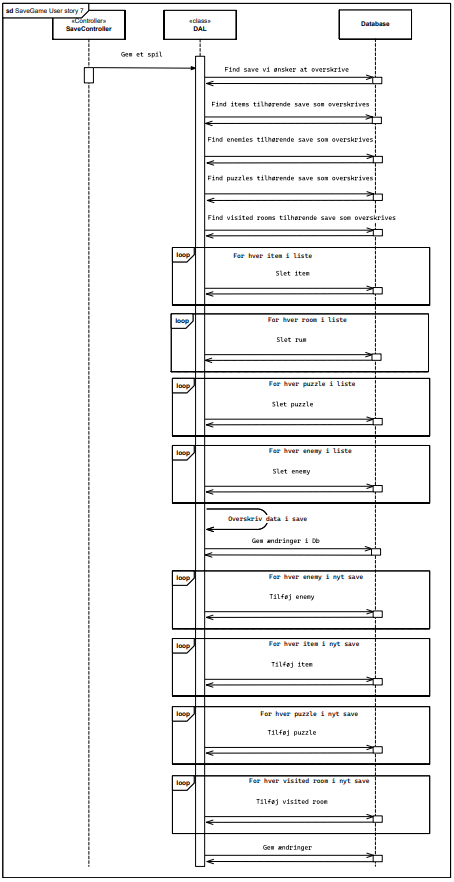
\includegraphics[width = 0.7\textwidth]{02-Body/Images/SaveGameDB.png}
\caption{Sekvensdiagram for User story 15: SaveGame. Dette diagram viser hvordan et spil gemmes}
\label{fig:SaveGameDB}
\end{figure}

På \autoref{fig:SaveGameDB}, SaveGame, ses der hvordan et spil vil gemmes. Måden dette vil fungere på er at spilleren vil starte med fem tomme gemte spil, som bliver seeded til databasen. Dette bliver gjort for at begrænse en bruger til fem gemte spil. Så for at gemme et spil findes der først hvilket gemte spil der skal overskrives. Derefter findes de relevante værdier i dette gemte spil. Hernæst slettes disse værdier og der tilføjes de nye korrekte værdier.\\
Brugeren vil derfor ikke have mulighed for at oprette et nyt spil, men kun mulighed for at overskrive en af fem tomme spil, som bliver oprettet for hver bruger.



\subsection{DAL Arkitektur}
I dette segment vil der blive forklaret tankerne bag arkitekturen vedr. oprettelsen af en funktionel DAL, som kan anvendes til at styre kommunikationen til og fra databasen.
Til oprettelsen af en funktionsdygtig database, i dette projekt, kræves der et relativt tæt sammenhold mellem databasen og backend api’en. API’en er ansvarlig for kommunikation mellem Front-end, Game Module og databasen.

\begin{figure}[H]
\centering
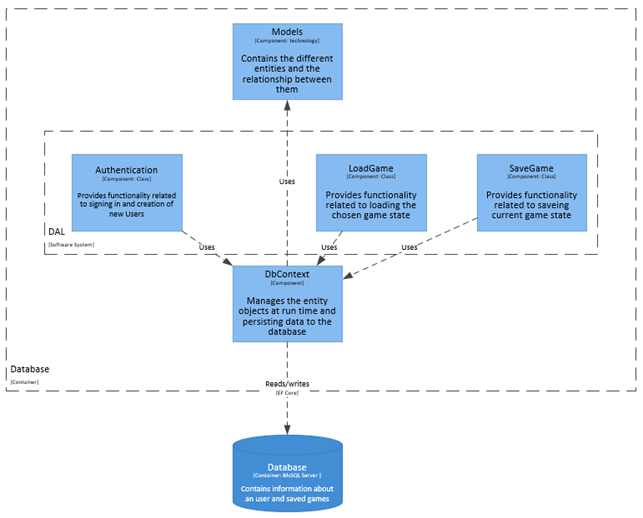
\includegraphics[width = \textwidth]{02-Body/Images/DALArkitektur}
\caption{C3 diagram for blokkene involveret i DAL's funktionalitet}

\label{fig:DALArkitektur}
\end{figure}


Når data enten skal sendes til eller hentes fra databasen så er det igennem et DAL. Systemets DAL giver os en simplificeret adgang til dataene gemt i databasen, og fungerer som en mellemmand for systemet, da alt kommunikation til databasen går igennem den.
I denne DAL har vi en Authentication, som bliver anvendt når en bruger logger ind, og når der oprettes en ny bruger. Denne blok kontrollerer brugernavn og kodeord, som sendes og hentes i databasen. Ydermere vil der ikke sættes fokus på sikkerhed, som ses i kravene stillet for systemet.
Yderligere vil det også være muligt at både gemme et spil og indlæse et spil. Begge af disse vil operere på det samme data, dog ville den ene, LoadGame, hente data fra systemets database, og den anden, SaveGame, vil sende data til systemets database. 
LoadGame i DAL er ansvarlig for at hente spillerens data fra databasen, såsom hvilket rum de var i og mængden af liv de har tilbage. 
Hernæst er der SaveGame. Denne indeholder funktionaliteten for at sende et gemt spil, altså dataene for spillerens nuværende spil. Heri vil der også gemmes information og spillerens nuværende tilstand i spillet. Det ville f.eks. være rummet som spilleren er i når spillet bliver gemt.
Begge af disse vil være ansvarlige for at håndtere data som er individuelle for hver spiller og hvert gemt spil.
Udenfor systemets DAL ville der også være inkluderet Models i konstruktionen af systemets database. Models vil indeholde de entities som Authentication og Load-/SaveGame vil bestå af. Yderligere vil Models også være ansvarlig for forholdene imellem de forskellige entities. 
